\documentclass[12pt,fleqn]{exam}
\usepackage{pifont}
\usepackage{dingbat}
\usepackage{amsmath,amssymb}
\usepackage{epsfig}
\usepackage[colorlinks=true,linkcolor=black,anchorcolor=black,citecolor=black,filecolor=black,menucolor=black,runcolor=black,urlcolor=black]{hyperref}
\usepackage[letterpaper, margin=0.75in]{geometry}
\addpoints
\boxedpoints
\pointsinmargin
\pointname{pts}

\usepackage[final]{microtype}
\usepackage[american]{babel}
%\usepackage[T1]{fontenc}
\usepackage{fourier}
\usepackage{isomath}
\usepackage{upgreek,amsmath}
\usepackage{amssymb}

\newcommand{\dotprod}{\, {\scriptzcriptztyle
    \stackrel{\bullet}{{}}}\,}

\newcommand{\reals}{\mathbf{R}}
\newcommand{\lub}{\mathrm{lub}} 
\newcommand{\glb}{\mathrm{glb}} 
\newcommand{\complex}{\mathbf{C}}
\newcommand{\dom}{\mbox{dom}}
\newcommand{\range}{\mbox{range}}
\newcommand{\cover}{{\mathcal C}}
\newcommand{\integers}{\mathbf{Z}}
\newcommand{\vi}{\, \mathbf{i}}
\newcommand{\vj}{\, \mathbf{j}}
\newcommand{\vk}{\, \mathbf{k}}
\newcommand{\bi}{\, \mathbf{i}}
\newcommand{\bj}{\, \mathbf{j}}
\newcommand{\bk}{\, \mathbf{k}}
\newcommand{\dist}{\, \mathrm{dist}}
\DeclareMathOperator{\Arg}{\mathrm{Arg}}
\DeclareMathOperator{\Ln}{\mathrm{Ln}}
\newcommand{\imag}{\, \mathrm{i}}

\usepackage{xcolor}
\shadedsolutions
\definecolor{SolutionColor}{rgb}{0.95,0.95,0.95}

\usepackage{graphicx}
\newcommand\AM{{\sc am}}
\newcommand\PM{{\sc pm}}
     
\usepackage{twemojis}
\newcommand{\quiz}{4}
\newcommand{\term}{Spring}
\newcommand{\due}{9:55 \AM}
\newcommand{\class}{MATH 102}
\begin{document}
\large
\vspace{0.1in}
\noindent\makebox[3.0truein][l]{\textbf{\class, \term \/ \the\year}}
\textbf{Name:} \hrulefill \\
\noindent \makebox[3.0truein][l]{\textbf{In class work \quiz}}
\textbf{Row and Seat}:\hrulefill\\
\vspace{0.1in}


\noindent  In class work  \quiz\/  has questions 1 through  \numquestions \/ with a total of  \numpoints\/  points.   
 This assignment is due at the end of the class period (\due).

\vspace{0.1in}


\begin{questions} 

\question The domain of a function $W$ is the closed interval $[-2,5]$
and its graph is shown below. Several dots on the graph are labeled for you.


    \begin{figure}[h]
        \begin{center}
        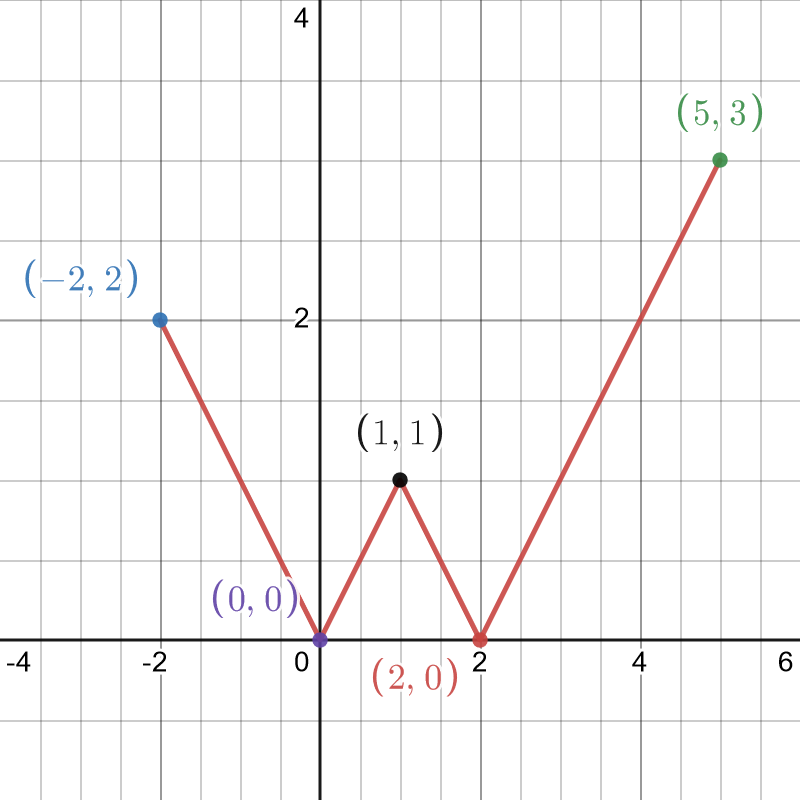
\includegraphics[scale=0.2]{desmos-graph(12).png}
    \end{center}
    \caption{Graph of the function $W$.}
    \end{figure}


\begin{parts}


    \part [1] Use the graph to determine the \emph{numerical value} of $W(1)$.
    \begin{solution}[1.0in]
    \end{solution}


    \part [1] Find the \emph{range} of $W$.  Remember that the range of
    a function is the set of all outputs. You need to collect all the 
    y coordinates that are on the graph.

    \begin{solution}[1.0in]
    \end{solution}

    \part[1] Find the interval(s) on which $W$ is \emph{decreasing}.
    \begin{solution}[1.0in]
    \end{solution}

    \part[1] Find the interval(s) on which $W$ is \emph{increasing}.
    \begin{solution}%[2.0in]
    \end{solution}




\end{parts}

\question The formula for a function $Q$ is $Q(x) = \max(1,x^2)$
and the domain of $Q$ is $[-3,3]$. A graph of $Q$ is shown below.

\begin{figure}[h]
    \begin{center}
    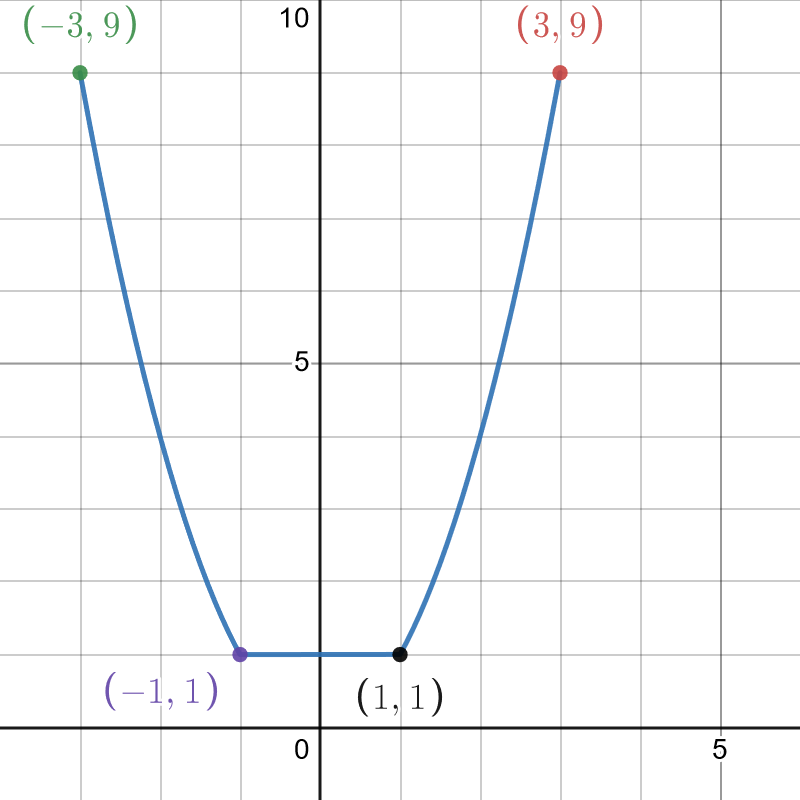
\includegraphics[scale=0.2]{desmos-graph(13).png}
\end{center}
\caption{Graph of the function $W$.}
\end{figure}

\begin{parts}

    \part[1] Find the interval on which $Q$ is a \emph{constant.}
    \begin{solution}[1.0in]
    \end{solution}


    \part [1] Find the average rate of change of $Q$ on the 
    interval $[-1,3]$. 


\end{parts}
\end{questions}
\end{document}